\documentclass[12pt]{article}
\usepackage[utf8]{inputenc} % UTF-8
\usepackage[T1]{fontenc}
\usepackage{lmodern} % Prévient un bug d'affichage evince lié à [T1]{fontenc}
\usepackage[frenchb]{babel} % francisation
\usepackage{adjustbox}
\usepackage[fleqn]{amsmath} % aligne le mode maths à gauche
\usepackage{amssymb} % the amsfont symbols
\usepackage[table, usenames, svgnames]{xcolor} % Couleurs
\usepackage{multicol} % Multi-colonnes
\usepackage{fancyhdr} % Mise en page, en-tête et pied de page
\usepackage{calc} % Opérations
\usepackage{marvosym} % Martin Vogels Symbole (\EUR)
\usepackage{cancel} % draw diagonal lines
\usepackage{units} % typesetting units and nice fractions
\usepackage[autolanguage]{numprint} % écrituredes virgules
\usepackage{tabularx} % creates a paragraph-like column whose width
                          % automatically expands
\usepackage{wrapfig} % allows figures or tables to have text wrapped around
\usepackage{pst-eucl, pst-plot} % figures géométriques
\usepackage{enumitem}
\usepackage{interval}
\usepackage{wasysym} % Symbole Euro
\usepackage{mathtools} % Encadrement dans align*
\usepackage[inline]{asymptote}
\usepackage{tkz-tab}
\usepackage{graphicx,float,grffile}

\usetikzlibrary{external} % set up externalization
\tikzexternalize[shell escape=-enable-write18] % activate externalisation
\tikzset{%
  external/system call={%
    latex \tikzexternalcheckshellescape -halt-on-error
    -interaction=batchmode -jobname "\image" "\texsource" &&
    dvips -o "\image".ps "\image".dvi &&
    ps2eps -f "\image.ps"
  }
}
\intervalconfig{ separator symbol={\,;\,}}

%\usepackage{textcomp}

\usepackage[a4paper, dvips, left=1.5cm, right=1.5cm, top=2cm,%
  bottom=2cm, marginpar=5mm, marginparsep=5pt]{geometry}
\newcounter{exo}
\frenchbsetup{StandardItemLabels} % remet \textbullet pour les listes
\setlength{\headheight}{18pt}
\setlength{\fboxsep}{5pt}
\setlength\parindent{0em}
\setlength\mathindent{0em}
\setlength{\columnsep}{30pt}
\usepackage[bookmarks=true, bookmarksnumbered=true, ps2pdf, pagebackref=true,%
            colorlinks=true,linkcolor=blue,plainpages=true,unicode]{hyperref}
\hypersetup{pdfauthor={Jérôme Ortais},pdfsubject={Exercices de
    mathématiques},pdftitle={Exercices créés par Pyromaths, un logiciel libre
    en Python sous licence GPL}}

\def\pshlabel#1{\psframebox*[fillcolor=White,framearc=.2]{\footnotesize $#1$}}
\def\psvlabel#1{\psframebox*[fillcolor=White,framearc=.2]{\footnotesize $#1$}}

\makeatletter
\newcommand\styleexo[1][]{
  \renewcommand{\theenumi}{\arabic{enumi}}
  \renewcommand{\labelenumi}{$\blacktriangleright$\textbf{\theenumi.}}
  \renewcommand{\theenumii}{\alph{enumii}}
  \renewcommand{\labelenumii}{\textbf{\theenumii)}}
  {\fontfamily{pag}\fontseries{b}\selectfont \underline{#1 \theexo}}
  \par\@afterheading\vspace{0.5\baselineskip minus 0.2\baselineskip}}
\newcommand*\exercice{%
  \psset{unit=1cm, dash=4pt 4pt, PointName=default,linecolor=Maroon,
    dotstyle=x, linestyle=solid, hatchcolor=Peru, gridcolor=Olive,
    subgridcolor=Olive, fillcolor=Peru}
  %\ifthenelse{\equal{\theexo}{0}}{}{\filbreak}
  \refstepcounter{exo}%
  \stepcounter{nocalcul}%
  \par\addvspace{1.5\baselineskip minus 1\baselineskip}%
  \@ifstar%
  {\penalty-130\styleexo[Corrigé de l'exercice]}%
  {\penalty-130\styleexo[Exercice]}%
  }
\newcommand{\checkedbox}[0]{\makebox[0pt][l]{$\square$}\raisebox{.15ex}{\hspace{0pt}$\checkmark$}}
\makeatother
\newlength{\ltxt}
\newsavebox{\mybox}
\newlength{\wdofmybox}
\newcommand{\figureadroite}[2]{%
  \setlength{\ltxt}{\linewidth}
  \sbox{\mybox}{\hbox{#1}}
  \settowidth{\wdofmybox}{\usebox{\mybox}}
  \addtolength{\ltxt}{-\wdofmybox}
  \addtolength{\ltxt}{-10pt}
  \begin{minipage}{\ltxt}
    #2
  \end{minipage}
  \hfill
  \begin{minipage}{\wdofmybox}
    #1
  \end{minipage}
}


\usepackage{fancyhdr} 
\pagestyle{fancyplain} 

\fancyhead{} % No page header
\fancyfoot{}

\renewcommand{\headrulewidth}{0pt} % Remove header underlines
\renewcommand{\footrulewidth}{0pt} % Remove footer underlines


\begin{document}

%----------------------------------------------------------------------------------------
% RE-DEFINITION
%----------------------------------------------------------------------------------------
% MATHS
%-----------

\newtheorem{Definition}{Définition}
\newtheorem{Theorem}{Théorème}
\newtheorem{Proposition}{Propriété}

% MATHS
%-----------
\renewcommand{\labelitemi}{$\bullet$}
\renewcommand{\labelitemii}{$\circ$}
\newcommand{\Pointilles}[1][3]{%
  \multido{}{#1}{\makebox[\linewidth]{\dotfill}\\[\parskip]
}}

%----------------------------------------------------------------------------------------
%	Titre
%----------------------------------------------------------------------------------------

\setlength{\columnseprule}{1pt}

\textbf{Nom, Prénom :} \hspace{8cm} \textbf{Classe :} \hspace{3cm} \textbf{Date :}\\
\vspace{-0.2cm}
\begin{center}
  \textit{L'art est comme un miroir, car il reflète notre âme.}  - \textbf{Alexandre Najjar}
\end{center}
\vspace{-0.2cm}


\subsection*{ex1 - DRILL}
\textbf{\textit{Calculer les longueurs, remplir le tableau, Les droites sont parallèles et les points sont alignés}}


\begin{figure}[H]
  \centering
  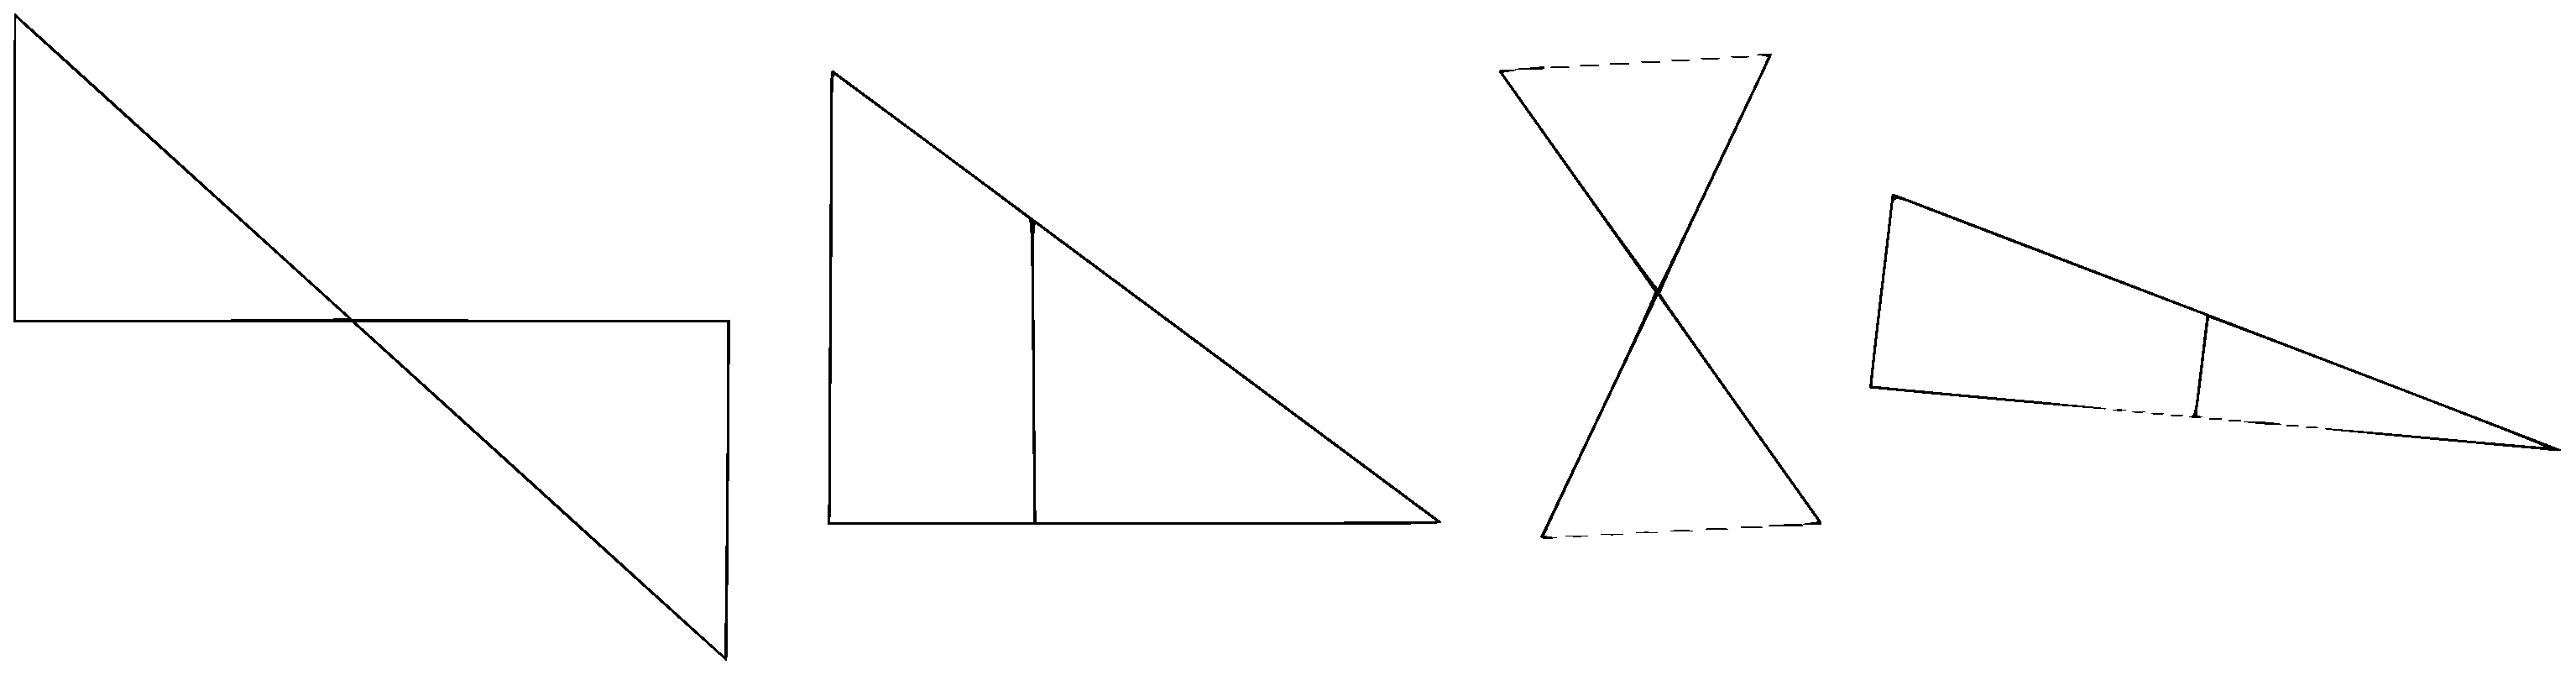
\includegraphics[width=0.9\linewidth]{3x5-thales/thales-ie.eps}
\end{figure}

\begin{multicols}{4}

  \begin{center}
    \begin{tabular}{|c|c|c|}
      \hline
      \phantom{azer} &  \phantom{azer} &  \phantom{azer} \\  \hline
      &  & \\  \hline
    \end{tabular}
  \end{center}

  \begin{center}
    \begin{tabular}{|c|c|c|}
      \hline
      \phantom{azer} &  \phantom{azer} &  \phantom{azer} \\  \hline
      &  & \\  \hline
    \end{tabular}
  \end{center}

  \begin{center}
    \begin{tabular}{|c|c|c|}
      \hline
      \phantom{azer} &  \phantom{azer} &  \phantom{azer} \\  \hline
      &  & \\  \hline
    \end{tabular}
  \end{center}


  \begin{center}
    \begin{tabular}{|c|c|c|}
      \hline
      \phantom{azer} &  \phantom{azer} &  \phantom{azer} \\  \hline
      &  & \\  \hline
    \end{tabular}
  \end{center}

\end{multicols}


\subsection*{ex2 - Calculer des longueurs}

  \figureadroite{%
  \psset{PointSymbol=none,unit=0.44}
  \begin{pspicture}(-1.5,-1.5)(7.53,4.54)
    \SpecialCoor
    \pstTriangle[PosAngleA=225, PosAngleB=-45, PosAngleC=106.85, PointNameA=S, PointNameB=C, PointNameC=Y](0,0){a}(6.03,0){b}(4.59;61.85){c}
    \pstTriangle[PosAngleB=-45, PosAngleC=151.85, PointSymbolA=none, PointNameA=none, PointNameB=M, PointNameC=F](0,0){a}(4.2,0){b}(3.2;61.85){c}
  \end{pspicture}
  }{%
    Sur la figure ci-contre, les droites $(CY)\text{ et }(MF)$ sont parallèles.\par
    On donne $SY=\unit[4{,}6]{cm}$ \quad $CY=\unit[5{,}6]{cm}$ \quad $SM=\unit[4{,}2]{cm}$ \quad $MF~=~\unit[3{,}9]{cm}$.\par
    Calculer $SC$ et $SF$.
  }\par
  \figureadroite{%
  \psset{PointSymbol=none,unit=0.26}
  \begin{pspicture}(-5.3,-3.65)(9.8,5.21)
    \SpecialCoor
    \pstTriangle[PosAngleA=135, PosAngleB=-45, PosAngleC=89.74, PointNameA=R, PointNameB=M, PointNameC=F](0,0){a}(8.3,0){b}(6.7;44.74){c}
    \pstTriangle[PosAngleB=135, PosAngleC=224.74, PointSymbolA=none, PointNameA=none, PointNameB=H, PointNameC=A](0,0){a}(-3.8,0){b}(-3.06;44.74){c}
  \end{pspicture}
  }{%
    Sur la figure ci-contre, les droites $(MF)\text{ et }(HA)$ sont parallèles.\par
    On donne $RF=\unit[6{,}7]{cm}$ \quad $MF=\unit[5{,}9]{cm}$ \quad $RH=\unit[3{,}8]{cm}$ \quad $HA~=~\unit[2{,}7]{cm}$.\par
    Calculer $RM$ et $RA$.
  }\par

\subsection*{ex3 - Parallélisme}

{\begin{wrapfigure}{r}{4cm}
  \psset{PointSymbol=none,unit=0.25}
  \begin{pspicture}(-1.5,-1.5)(14.3,5.94)
    \SpecialCoor
    \pstTriangle[PosAngleA=225,PosAngleB=-45,PosAngleC=72,PointNameA=E,PointNameB=Y,PointNameC=H](0,0){a}(12.8,0){b}(12.0;27){c}
    \pstTriangle[PosAngleB=-45,PosAngleC=117,PointSymbolA=none,PointNameA=none,PointNameB=R,PointNameC=I](0,0){a}(8.0,0){b}(7.5;27){c}
  \end{pspicture}
  \end{wrapfigure}\par
  
    Sur la figure ci-contre, on donne $EY=\unit[12{,}8]{cm}$, $EH=\unit[12]{cm}$, $RY=\unit[4{,}8]{cm}$ et $EI=\unit[7{,}5]{cm}$.\par
    Démontrer que les droites $(YH)$ et $(RI)$ sont parallèles.
  \vspace{2cm}}

  {\begin{wrapfigure}{r}{4cm}
    \psset{PointSymbol=none,unit=0.48}
    \begin{pspicture}(-1.5,-1.5)(5.5,6.68)
      \SpecialCoor
      \pstTriangle[PosAngleA=225,PosAngleB=-45,PosAngleC=120,PointNameA=W,PointNameB=U,PointNameC=C](0,0){a}(4.0,0){b}(6.4;75){c}
      \pstTriangle[PosAngleB=-45,PosAngleC=165,PointSymbolA=none,PointNameA=none,PointNameB=Z,PointNameC=H](0,0){a}(1.5,0){b}(2.4;75){c}
    \end{pspicture}
    \end{wrapfigure}\par
    
      Sur la figure ci-contre, on donne $WZ=\unit[1{,}5]{cm}$, $WH=\unit[2{,}4]{cm}$, $WU=\unit[4]{cm}$ et $HC=\unit[4]{cm}$.\par
      Démontrer que les droites $(UC)$ et $(ZH)$ sont parallèles.
    \vspace{2cm}}

\newpage

\textbf{Nom, Prénom :} \hspace{8cm} \textbf{Classe :} \hspace{3cm} \textbf{Date :}\\
\vspace{-0.2cm}
\begin{center}
  \textit{L'art est comme un miroir, car il reflète notre âme.}  - \textbf{Alexandre Najjar}
\end{center}
\vspace{-0.2cm}


\subsection*{ex1 - DRILL}
\textbf{\textit{Calculer les longueurs, remplir le tableau, Les droites sont parallèles et les points sont alignés}}


\begin{figure}[H]
  \centering
  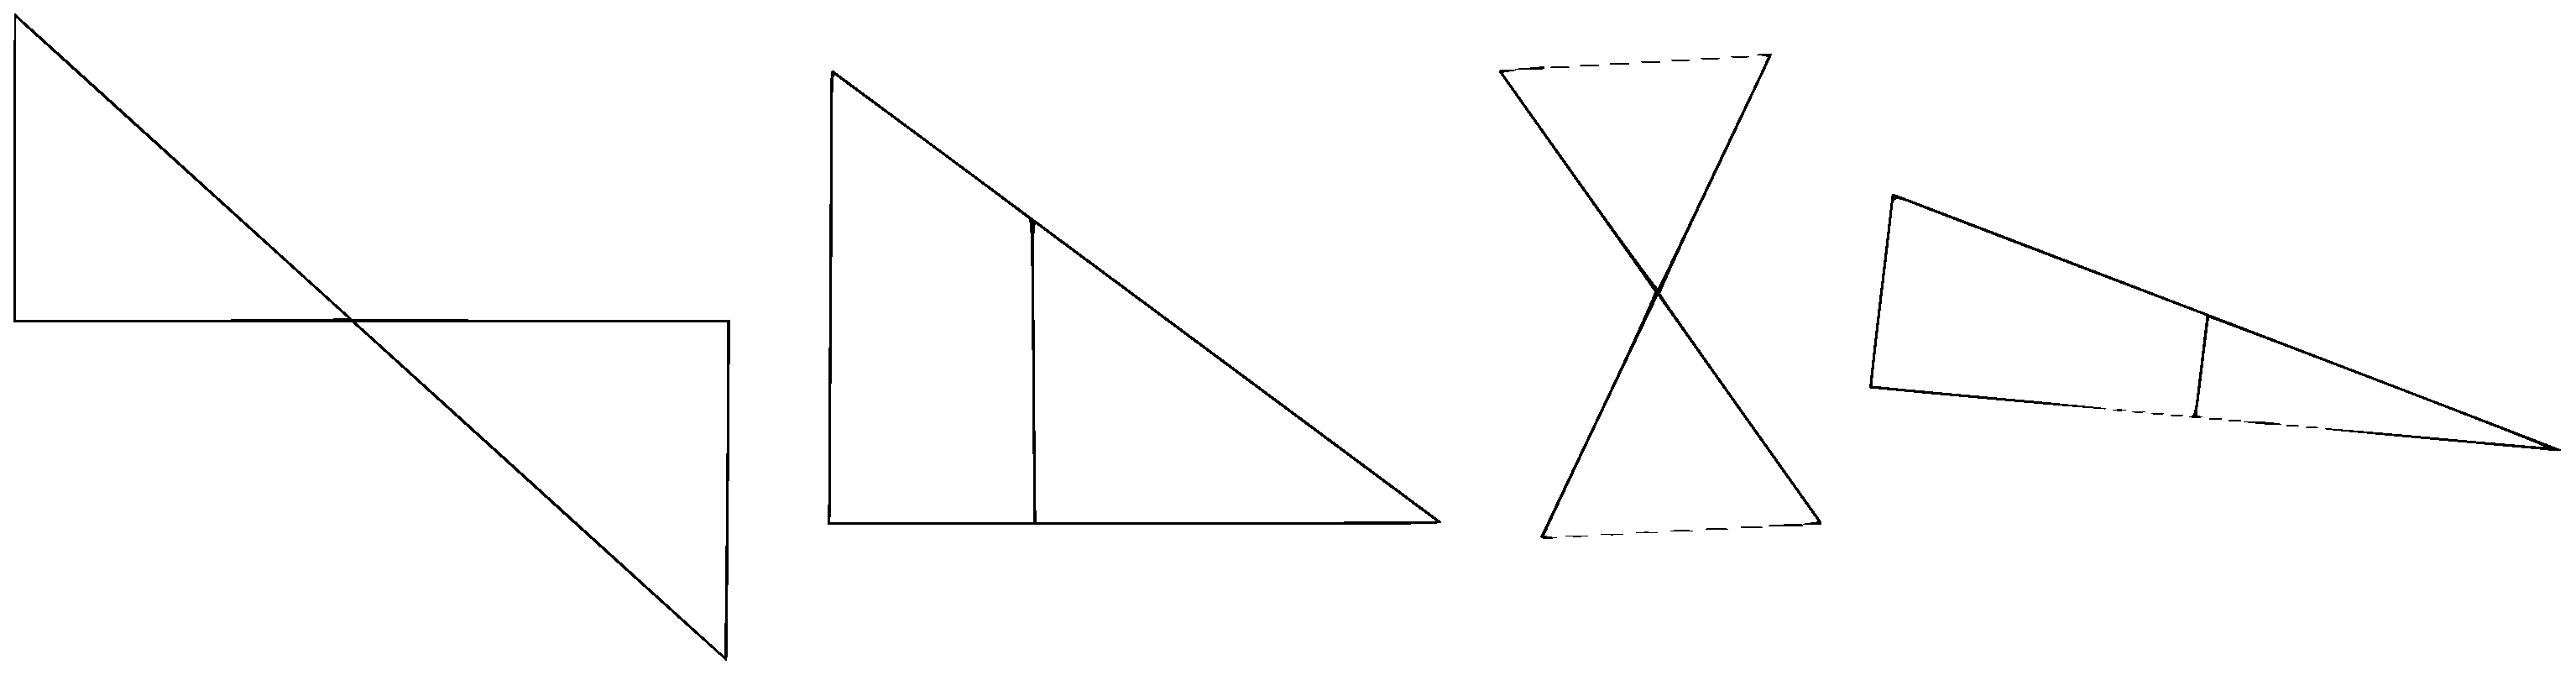
\includegraphics[width=0.9\linewidth]{3x5-thales/thales-ie.eps}
\end{figure}

\begin{multicols}{4}

\begin{center}
  \begin{tabular}{|c|c|c|}
    \hline
    \phantom{azer} &  \phantom{azer} &  \phantom{azer} \\  \hline
     &  & \\  \hline
  \end{tabular}
\end{center}

\begin{center}
  \begin{tabular}{|c|c|c|}
    \hline
    \phantom{azer} &  \phantom{azer} &  \phantom{azer} \\  \hline
     &  & \\  \hline
  \end{tabular}
\end{center}

\begin{center}
  \begin{tabular}{|c|c|c|}
    \hline
    \phantom{azer} &  \phantom{azer} &  \phantom{azer} \\  \hline
     &  & \\  \hline
  \end{tabular}
\end{center}


\begin{center}
  \begin{tabular}{|c|c|c|}
    \hline
    \phantom{azer} &  \phantom{azer} &  \phantom{azer} \\  \hline
     &  & \\  \hline
  \end{tabular}
\end{center}

\end{multicols}


\subsection*{ex2 - Calculer des longueurs}
\figureadroite{%
\psset{PointSymbol=none,unit=0.39}
\begin{pspicture}(-3.4299999999999997,-2.67)(6.62,3.61)
  \SpecialCoor
  \pstTriangle[PosAngleA=135, PosAngleB=-45, PosAngleC=76.26, PointNameA=K, PointNameB=O, PointNameC=L](0,0){a}(4.5,0){b}(6.0;31.26){c}
  \pstTriangle[PosAngleB=135, PosAngleC=211.26, PointSymbolA=none, PointNameA=none, PointNameB=J, PointNameC=R](0,0){a}(-1.7,0){b}(-2.26;31.26){c}
\end{pspicture}
}{%
  Sur la figure ci-contre, les droites $(OL)\text{ et }(JR)$ sont parallèles.\par
  On donne $KL=\unit[6]{cm}$ \quad $KJ=\unit[1{,}7]{cm}$ \quad $JR=\unit[1{,}2]{cm}$ \quad $JO~=~\unit[6{,}2]{cm}$.\par
  Calculer $OL$ et $KR$.
}\par
\figureadroite{%
\psset{PointSymbol=none,unit=0.62}
\begin{pspicture}(-1.5,-1.5)(4.85,2.05)
  \SpecialCoor
  \pstTriangle[PosAngleA=225, PosAngleB=-45, PosAngleC=69.93, PointNameA=L, PointNameB=E, PointNameC=G](0,0){a}(3.0,0){b}(3.7;24.93){c}
  \pstTriangle[PosAngleB=-45, PosAngleC=114.93, PointSymbolA=none, PointNameA=none, PointNameB=N, PointNameC=D](0,0){a}(0.93,0){b}(1.15;24.93){c}
\end{pspicture}
}{%
  Sur la figure ci-contre, les droites $(EG)\text{ et }(ND)$ sont parallèles.\par
  On donne $LE=\unit[3]{cm}$ \quad $LG=\unit[3{,}7]{cm}$ \quad $EG=\unit[1{,}6]{cm}$ \quad $ND~=~\unit[0{,}5]{cm}$.\par
  Calculer $LN$ et $LD$.
}\par


\subsection*{ex3 - Parallélisme}

{\begin{wrapfigure}{r}{4cm}
  \psset{PointSymbol=none,unit=0.28}
  \begin{pspicture}(-2.7,-5.68)(3.7,8.18)
    \SpecialCoor
    \pstTriangle[PosAngleA=135,PosAngleB=-45,PosAngleC=131,PointNameA=K,PointNameB=M,PointNameC=G](0,0){a}(2.2,0){b}(7.7;86){c}
    \pstTriangle[PosAngleB=135,PosAngleC=266,PointSymbolA=none,PointNameA=none,PointNameB=L,PointNameC=D](0,0){a}(-1.2,0){b}(-4.2;86){c}
  \end{pspicture}
  \end{wrapfigure}\par
  
    Sur la figure ci-contre, on donne $KG=\unit[7{,}7]{cm}$, $KM=\unit[2{,}2]{cm}$, $KD=\unit[4{,}2]{cm}$ et $LM=\unit[3{,}4]{cm}$.\par
    Démontrer que les droites $(MG)$ et $(LD)$ sont parallèles.
  \vspace{2cm}}

{\begin{wrapfigure}{r}{4cm}
  \psset{PointSymbol=none,unit=0.4}
  \begin{pspicture}(-1.5,-1.5)(8.280000000000001,5.61)
    \SpecialCoor
    \pstTriangle[PosAngleA=225,PosAngleB=-45,PosAngleC=82,PointNameA=O,PointNameB=N,PointNameC=A](0,0){a}(5.1,0){b}(8.5;37){c}
    \pstTriangle[PosAngleB=-45,PosAngleC=127,PointSymbolA=none,PointNameA=none,PointNameB=R,PointNameC=H](0,0){a}(2.4,0){b}(4.0;37){c}
  \end{pspicture}
 \end{wrapfigure}\par
    
    Sur la figure ci-contre, on donne $OA=\unit[8{,}5]{cm}$, $ON=\unit[5{,}1]{cm}$, $OR=\unit[2{,}4]{cm}$ et $HA=\unit[4{,}5]{cm}$.\par
    Démontrer que les droites $(NA)$ et $(RH)$ sont parallèles.
  \vspace{2cm}}

\end{document}
